\documentclass{article}

\usepackage{physics} % Handy shortcuts like \pdv, \dd and much more
\usepackage{geometry} % smaller margins, can be adjusted if given arguments
\usepackage{siunitx} % the \si environment for units
\usepackage{mathtools} % The dcases environment, prettier than just cases
\usepackage{tikz} % For drawing picures
\usepackage{wrapfig} % Wrapping text around figures


\title{Exercise 1 - TFY4345 Classical Mechanics}
\date{2020}

\begin{document}
    \maketitle
    \section{Halley's comet}
        Halley's comet follows an elliptical orbit around the Sun, with a period of about 76 years. The sun is a focal point in the ellipse. The closest distance between the comet an the sun is $\SI{0.6}{AU}$, and the farthest distance is $ \SI{35}{AU}$. $\SI{1}{AU}$ (astronomical unit) is the mean distance between the Sun and the earth. Use the Sun as the origin in your coordinate system. \\ \\
        (a) Explain why the net torque on Halley's comet is zero. This implies that the angular momentum is conserved \\ \\
        (b) When the comet is closest to the Sun, it's velocity is $\SI{54}{km.\per.s}$. Use conservation of angular momentum to calculate the velocity of the comet when it is farthest from the Sun.

    \section{Simple pendulum}
        \begin{wrapfigure}{2}{0.4\textwidth}
            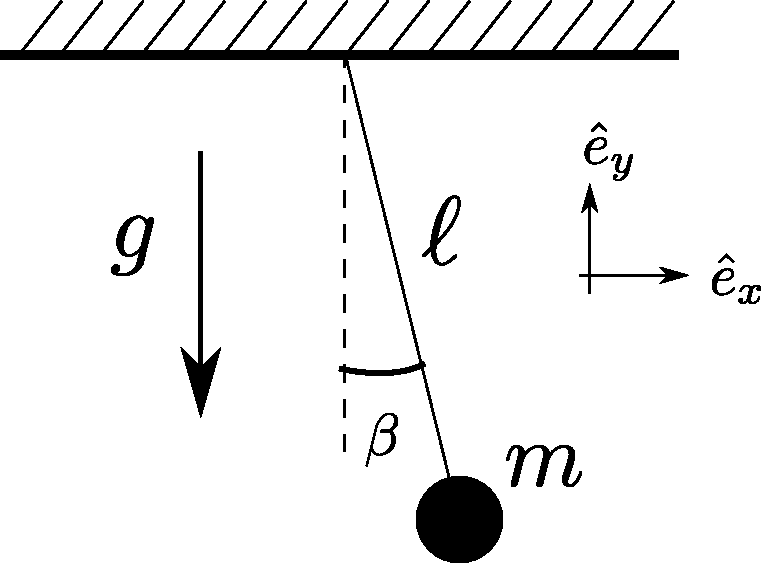
\includegraphics[width=0.4\textwidth]{figures/figure_1.pdf}
        \end{wrapfigure}
        Consider a simple pendulum, subject to a uniform gravitational field $\vec{g} = -g \hat e_x$ Chose the pivot point as the origin of your coordinate system There are no friction forces. \\ \\
        (a) Show that the position vector of the mass $m$ is $\vec R = \ell \sin(\beta) \hat e_x - \ell \cos(\beta) \hat e_y$.  \\ \\
        (b) Find the potential energy of the mass, as a function of the angle $\beta$. \\ \\
        (c) Find the kinetic energy of the mass, as a function of $\beta$ and $\dot \beta = \dv{\beta}{t}$. \\ \\
        (d) The Lagrangian of the pendulum is $L = T - V$. Use Lagrange's equations to obtain the equation of motion of the pendulum.
        \newpage

    \section{Double pendulum}
        \begin{wrapfigure}{2}{0.4\textwidth}
            \vspace{-1cm}
            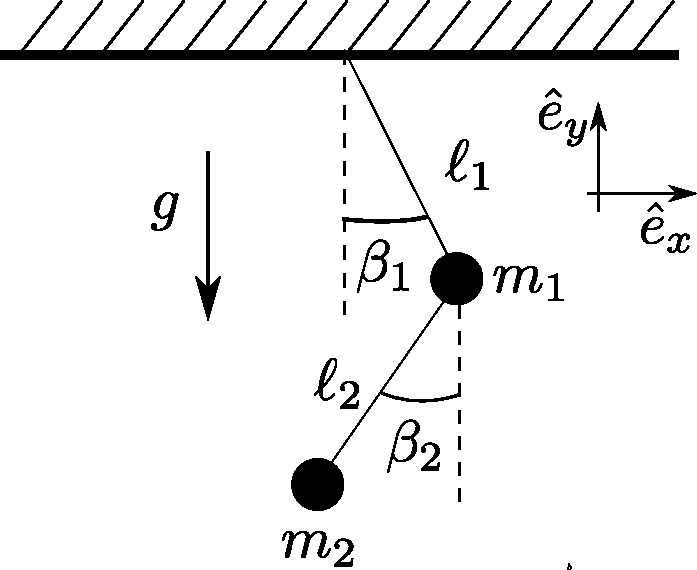
\includegraphics[width=0.4\textwidth]{figures/figure_2.pdf}
            \vspace{-2cm}
        \end{wrapfigure}
        (a) Find the Lagrangian $L = T - V$ for the coplanar \footnote{coplanar objects are objects in the same plane} double pendulum in a uniform gravitational field. Choose the angles $\beta_1$, $\beta_2$ as the coordinates. \\ \\
        (b) Obtain the equations of motion using the Lagrange equations.

    \section{Lagrangian invariance}
        Show by direct substitution that the transformed Lagrangian
        \begin{equation*}
            L'(q, \dot q, t) = L(q, \dot q, t) + \dv{F(q, t)}{t},
        \end{equation*}
        where $F$ is an arbitrary function of $q, t$ leads to the same equations of motion (the Lagrange equations) as the original Lagrangian $L(q, \dot q, t)$.\\  \\
        (Hint: Start from the Lagrange equations and use the chain rule for partial derivatives for the function $F(q, t)$)

\end{document}

